\documentclass[12pt,a4paper]{article}
\usepackage[T1]{fontenc}
\usepackage[a4paper]{geometry}
\usepackage[portuges,brazilian]{babel}
\usepackage[utf8]{inputenc}
\usepackage{setspace}
\usepackage{libertine}
\usepackage{graphicx}	
\usepackage{ragged2e} 
\usepackage{authblk}
\usepackage{hyperref}		
%
\newcommand*{\email}[1]{%
    \normalsize\href{mailto:#1}{#1}\par
    }


\begin{document} 
\begin{figure}
    \flushright
    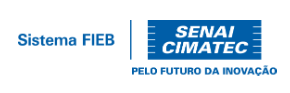
\includegraphics[scale=0.5]{Logo_senai.png}
\end{figure}

\title{Roteiro \\ Robôs de Segurança de patrimônio} 
\author{Anderson Queiroz}
\affil{Senai Cimatec. CCRoSA - Centro de Competência em Robótica e Sitemas Autônomos \\ \email{anderson.vale@fbter.org.br}}

 

    \maketitle
    \pagenumbering{arabic}
    \singlespacing


    


\end{document}